\documentclass{uflamon}          % classe base para a monografia

%==============================================================================
% Utilizacao de pacotes
\usepackage[T1]{fontenc}         % usa fontes postscript com acentos
\usepackage[brazil]{babel}       % hifenização e títulos em português do Brasil
\usepackage[utf8]{inputenc}     % permite edição direta com acentos
\usepackage{amsmath}             % pacote da AMS para Matemática Avançada
\usepackage{amssymb}             % símbolos extras da AMS
\usepackage{latexsym}            % símbolos extras do LaTeX
\usepackage{graphicx}            % para inserção de gráficos
\usepackage{listings}            % para inserção de código
\usepackage{fancyvrb}            % para inserção de saídas de comandos
%\usepackage{enumerate}           % para personalizar lista enumeradas 
											%(incluso na classe)
\usepackage{longtable}           % para tambelas muito grandes NOVO!!!!

\usepackage{colortbl} % cores em tabelas
\newcolumntype{Z}{|>{\columncolor[gray]{0.9}}l|} %cor cinza em células
%\usepackage{array} % já incluso na classe
\newcolumntype{L}[1]{>{\raggedright\let\newline\\\arraybackslash\hspace{0pt}}m{#1}}
\newcolumntype{C}[1]{>{\centering\let\newline\\\arraybackslash\hspace{0pt}}m{#1}}
\newcolumntype{R}[1]{>{\raggedleft\let\newline\\\arraybackslash\hspace{0pt}}m{#1}}
\usepackage{multirow} % para juntar duas linhas em uma só
\usepackage{multicol} % para uso de várias colunas
%\usepackage{subfig}

% cores para os links cruzados
\usepackage{color}
\definecolor{rltred}{rgb}{0.2,0,0}
\definecolor{rltgreen}{rgb}{0,0.2,0}
\definecolor{rltblue}{rgb}{0,0,0.2}

\usepackage[colorlinks=true,
            urlcolor=rltblue,       % \href{...}{...} external (URL)
            filecolor=rltgreen,     % \href{...} local file
            linkcolor=black,       % \ref{...} and \pageref{...}
            citecolor=black,
            pdftitle={Filtro Prensa},
          pdfauthor={Marcus Bruno Fernandes Silva},
          pdfsubject={Planta Piloto de Filtro Prensa},
          pdfkeywords={filtro prensa}%
]{hyperref} % para referência cruzadas
%\usepackage{hyperref}            % para referência cruzadas
\usepackage{subfigure}           % figuras dentro de figuras
\usepackage{caption}            % remodelando o formato dos títulos de 
                                 % tabelas e figuras

% configuração padrão do listings   
\lstset{%
   language=Java,
   extendedchars=true,
   tabsize=3,
   basicstyle=\footnotesize\ttfamily,
   stringstyle=\em,
   showstringspaces=false 
}

%abnt-emphasize=bf coloca o título das bibliografias em negrito
%abnt-thesis-year=both
\usepackage[alf,num,abnt-etal-cite=3,abnt-etal-list=3,abnt-url-package=url,abnt-emphasize=bf]{abntex2cite}

% redefinindo formatação de títulos de tabelas e figuras

%==============================================================================
\usepackage{microtype} 			% para melhorias de justificação
\usepackage{float}
\usepackage{titling}
\usepackage[version=4]{mhchem}
\usepackage{array}
\usepackage{siunitx}
\usepackage{enumitem}
\usepackage{booktabs}
% \usepackage{nameref} % Referencia capitulos por nome
%\usepackage[authoryear]{natbib}

% Especificando hifenizações que por ventura LaTeX não saiba fazer
% Por padrão 99,9% dos termos em português devem ser hifenizados corretamente.
\hyphenation{hardware software Li-nux am-bien-te diag-nos-ti-car coor-de-na-ção 
  FAE-PE Recovery TelEduc Williams UFLA Sérgio Renata Reynolds disciplina Iara
Hernandez Rodrigues}

%==============================================================================
% Dados da monografia, capa: autor, titulo, banca, etc... - SUBSTITUA DE ACORDO
%==============================================================================
\author{Gabriela Nunes \\
        Gustavo Henrique de Souza Paiva \\
        Karen Leticia Sanchez Costa \\
        Larissa Souza Castro \\
        Marcus Bruno Fernandes Silva \\
        Marina Leticia Alves Ferreira}
\subtitle{Exemplo para os Usuários}
%\author{Joao}
\title{Planta Piloto de Filtro Prensa}
\engtitle{Use of Uflamon Class}
%\engsubtitle{Sample for Users}
%\edicao{3$^a$ edição revista, atualizada e ampliada}
\date{2017}
\newcommand{\orient}{Professora Iara Hernandez Rodriguez}
\newcommand{\disciplina}{GNE340}
\tipo{Projeto entregue e apresentado à \orient{} como requisito da disciplina \disciplina{}.}
\orientador{\orient}
\newcommand{\otipo}{Projeto entregue e apresentado à \orient{} como requisito da disciplina \disciplina{}.}
\newcommand{\olocal}{Lavras -- MG}
\local{Lavras -- MG}

%##################################################

\newcommand \fazercapa{
\begin{titlepage}
    \centering

    
\includegraphics[scale=0.45]{logoufla.jpg}%

    \vspace{1cm}

    \Large\theauthor
    
    \vspace{\stretch{1}}

    \bfseries\LARGE\MakeUppercase\thetitle

    \vspace{\stretch{1}}

    \Large\MakeUppercase\olocal\\
    \MakeUppercase\thedate
    \null
    \cleardoublepage
\end{titlepage}
}

\newcommand \fazerfolhaderosto{
    \begin{titlepage}
        \newpage

        \begin{center}
            \MakeUppercase\theauthor

            \vspace{\stretch{1}}

            \textbf{\MakeUppercase\thetitle}

            \vspace{\stretch{1}}
            
            \hfill\begin{minipage}{8cm}{\otipo}\end{minipage} % tipo da monografia

            \vspace{\stretch{.58}}

            \ifthenelse{\equal{\@orientador}{\@empty}} % % se orientador nao existir,
            {}%                                            % nao produza nada
            {\orient\\
             Orientadora
            }

            \vspace{\stretch{.86}} 

            \textbf{\MakeUppercase\olocal}\\ 
            \textbf{\MakeUppercase\thedate}
            \end{center}
    \end{titlepage}
}

\newcolumntype{P}[1]{>{\centering\arraybackslash}p{#1}}
\graphicspath{{./figuras/}}

\newcommand{\tabitem}{~~\llap{\textbullet}~~}
\newcommand{\R}{$^{\tiny{\textregistered}}$~}


%==============================================================================

% Meus comandos

\newcommand{\citeay}[1]{\citeauthoronline{#1} (\citeyear{#1})}
\newcommand{\citeayp}[1]{(\citeauthoronline{#1} \citeyear{#1})}
\newcommand{\citean}[1]{\citeauthoronline{#1} \cite{#1}}
\newcommand{\pa}[1]{\left(#1 \right)}

%==============================================================================
% Começar o documento

%\newsubfloat{figure}

%\includeonly{capitulos/materiais_metodos,capitulos/resultados}
\begin{document}

\fazercapa

\fazerfolhaderosto

\tableofcontents

\clearpage

\pagestyle{ufla}

%==============================================================================
% incluindo os capitulos


\chapter{Introdução} \label{sec:intro}

\section{Referencial Teórico}\label{sec:refteo}

Reaproveitar materiais e fazer de seu novo uso algo útil, não só é tendência,
como algo necessário, pois com o avanço tecnológico e crescimento populacional,
a preocupação com os recursos naturais tende a aumentar. Reutilizar recipientes
metálicos para construir um filtro, além de evitar deposição de materiais no
meio ambiente, como poluentes, pode ser uma alternativa de baixo custo para
tratamento de água, antes de despejá-la em efluentes, unindo desenvolvimento de
tecnologia de baixo custo e funcionalidade com preservação do meio ambiente.

Um dos procedimentos mais simples de separação de sólidos e líquidos é a
filtração, aplicada em muitas etapas de processos da indústria química. Entra no
filtro a mistura a ser separada e como produtos, saem o filtrado (líquido
clarificado) e a torta de filtragem (sólido com um pouco de líquido). Ao longo
do processo, a própria torta se torna o meio filtrante, e como no início ela
está sendo formada, para que seja efetiva a filtração, os volumes iniciais
retornam ao filtro. Durante a filtração, características como altura,
permeabilidade e porosidade da torta, variam, também há variação de pressão ao
longo do processo, alterando a vazão. As variáveis devem ser controladas para
cálculo da velocidade da filtração e consequentemente o tempo gasto, sempre
buscando otimizar o processo \citeayp{isenmann2012operaccoes} .

\subsection{Tipos de filtro}

\label{subsec:tiposdefiltro}

\begin{enumerate}

\item[-] Filtro de pressão
 
  São filtros que funcionam em batelada, ou de forma contínua, operam
  pressurizados e costumam ter uma ou mais camadas de material granular. São
  usados geralmente em estações de tratamento de água. O filtro prensa é deste
  tipo, tem como vantagens a necessidade de uma menor área para sua implantação,
  São produzidos líquidos límpidos por meio da circulação do filtrado, as tortas
  resultantes apresentam baixa umidade e pode ser automatizado. Porém, tem as
  desvantagens de difícil lavagem e manutenção, as placas podem sofrer fissuras
  e romper-se e a técnica é muito sensível às variações das características dos
  resíduos \citeayp{Cremasco14}.


\item[-] Filtro a vácuo

  Ainda, segundo \citeay{Cremasco14}, os filtros a vácuo podem ser alimentados
  no fundo ou no topo do equipamento. Caracteriza-se por conduzir tortas secas
  de pequena espessura, e operar continuamente sob baixa queda de pressão. É
  utilizado na indústria sucroalcooleira, no modelo contínuo de tambor rotativo
  a vácuo, por exemplo. Suas tortas apresentam maior quantidade de umidade
  residual se comparado ao filtro prensa, o meio filtrante requer lavagem
  constante e consome bastante energia, mas em compensação, a unidade precisa de
  pequena área de implantação, a torta é facilmente removível, tem fácil
  controle operacional e manutenção de baixo custo.


\end{enumerate}


\subsection{Meios filtrantes}
\label{subsec:meiosfiltrantes}

Para escolher um meio filtrante, precisam ser analisadas anteriormente
características que serão essenciais na otimização da filtração. É importante
que ao entrar em contato com a suspensão que será tratada, o meio filtrante não
sofra fissuras, rompimentos ou ataques químicos. Ter boa e adequada distribuição
dos poros faz com que o curso da filtração não seja comprometido, seja fácil
fazer a limpeza e o custo seja baixo \citeayp{Cremasco14}.

Após o início da operação, a torta se tornará meio filtrante, por isso, para
obter filtrado límpido, é importante voltar os primeiros volumes ao processo,
visto que nas primeiras porções de filtrado há traços de particulado.

Alguns meios utilizados que merecem ser citados são algodão, polímeros
sintéticos, metais, e no caso de filtros granulares, cascalho, areia, antracito
e carvão ativado \citeayp{Cremasco14}.


\subsection{Fluidodinâmica da filtração}

Existem dois tipos de filtração granular: rápida e lenta. Na filtração rápida,
as partículas apresentam-se diluídas na suspensão e não apresentam interação com
o material filtrante, de modo a não obstruir os poros do material granular. Na
filtração lenta, a remoção de partículas em suspensão depende de interações
entre os sólidos e o meio filtrante (forças repulsivas e atrativas, e mecanismos
como a difusão e exclusão por tamanho, sendo a abordagem microscópica
caracterizada por considerar esses mecanismos; e a macroscópica, por
desconsiderá-los) \citeayp{Cremasco14}.

A descrição generalizada pode ser visualizada na Tabela \ref{table:fluidodinamicafiltracao}:

\newcommand{\tbu}{\textbf{u}}
\begin{table}[H]
\centering
\caption{Descrição da fluidodinâmica da filtração \citeayp{Cremasco14}}
\label{table:fluidodinamicafiltracao}
\resizebox{\textwidth}{!}{
\begin{tabular}{p{2.4cm}l}
\toprule
Equação da continuidade da fase fluida      & $ \pderr{\rho\varepsilon}{t}+\vec{\nabla}\cdot(\rho\varepsilon \tbu{}) = -\phi$\\[1.4cm]
Equação da continuidade da fase particulada & $ \pderr{\rho_p\varepsilon_p}{t}+\vec{\nabla}\dot(\rho_p\varepsilon_p \tbu{}_p) = \phi$\\[1.4cm]
Equação do movimento da fase fluida         & $ \pderr{\rho\varepsilon\tbu{}}{t}+\vec{\nabla}\cdot(\rho\varepsilon\tbu{}\tbu{})=\vec{\nabla}\cdot\textbf{T}-\beta(\tbu{}-\tbu{}_p)+\rho\textbf{b}$\\[1.4cm]
Equação do movimento da fase particulada    & $ \pderr{\rho_p\varepsilon_p\tbu{}_p}{t}+\vec{\nabla}\cdot(\rho_p\varepsilon_p\tbu{}_p\tbu{}_p)=\vec{\nabla}\cdot\textbf{T}_p-\beta(\tbu{}-\tbu{}_p)+\varepsilon_p(\rho_p-\rho)\textbf{b}$\\\bottomrule
\end{tabular}
}
\end{table}

Na Tabela \ref{table:fluidodinamicafiltracao} o termo de campo \textbf{b} será
definido a medida que se adotar qual filtro será utilizado na operação:
gravitacional ou rotativo, por exemplo. Já a grandeza $\phi$ refere-se ao fluxo
de captura, por meio do material, nas partículas presentes na suspensão a ser
filtrada. Deve-se considerar essa grandeza quando há filtração lenta em filtro
granular, na filtração granular rápida e filtração com ou sem formação de torta
deformável essa grandeza não deve ser considerada \citeayp{Cremasco14}. Conforme
o autor, esse parâmetro pode ser representado das seguintes formas:

\begin{enumerate}
\item[] Abordagem microscópica
  \begin{equation}
    \phi = D_{ef} \nabla^2(\rho_p\varepsilon_p)
  \end{equation}
  
\item[] Abordagem macroscópica
  \begin{equation}
    \phi = \pa{\frac{\rho_p\varepsilon_p}{\delta}}\tbu{}\lambda
  \end{equation}
\end{enumerate}

O tensor tensão da fase fluida, \textbf{T}, é descrito pela componente de
pressão, $p$, nesta fase:

\begin{equation}
  \label{eq:tensortensao}
  \textbf{T} = p \textbf{I}
\end{equation}

O coeficiente $\beta$, parâmetro de arraste, é referente à parcela da
contribuição Darcyniana do escoamento:
\begin{equation}
  \label{eq:parametroB}
  \beta = \frac{\mu\varepsilon}{k(\varepsilon)}
\end{equation}
onde $k(\varepsilon)$ pode ser obtido por correlações encontradas na literatura.

A descrição da fluidodinâmica da filtração depende de qual tipo de filtro será
utilizado, e também do conhecimento de informações, como: características
físicas e químicas das fases, reologia da suspensão e da natureza do meio
filtrante \citeayp{Cremasco14}.

\subsection{Filtração com formação de torta: teoria simplificada da filtração}

A operação de filtração de suspensões que resulta na formação de tortas
caracteriza-se por exibir variação de porosidade da matriz porosa (torta) ao
longo do tempo e da sua estrutura, causada pela percolação do fluido,
ocasionando o meio poroso deformável.

A formulação para a fluidodinâmica advém da análise da Tabela
\ref{table:fluidodinamicafiltracao}, considerando-se nula a contribuição do
fluxo de captura. São consideradas as seguintes hipóteses
\citeayp{massarani2001fluidodinamica}:

\begin{itemize}
\item[-] o tensor tensão da fase fluida é descrito pela componente de pressão;
\item[-] o valor da velocidade da fase particulada ser bem menor do que o valor
  da velocidade da fase fluida, assim a velocidade relativa $U$, fica sendo a
  velocidade do fluido.
\end{itemize}

Além disso, são estabelecidas as seguintes hipóteses para a filtração com formação de
torta \citeayp{Cremasco14}: 
\begin{itemize}
\item[-] a fase fluida comporta-se como fluido newtoniano e incompressível; 
\item[-] escoamento unidimensional de onde resulta, para a velocidade relativa:
  $$U = u = q/\varepsilon$$
  onde $u$ é a velocidade intersticial da fase fluida, $q$ é a velocidade
  superficial da fase fluida e $\varepsilon$ é a porosidade do meio filtrante.
\end{itemize}

Correlacionando os resultados da filtração com as condições operacionais,
expressas pela queda de pressão no filtro, considerando que a torta e o meio
filtrante são meios porosos percolados em série pelo fluido, e que a velocidade
superficial do fluido e a massa de sólido seco na torta estão relacionadas ao
volume de filtrado $V$, ao tempo $t$, à área de filtração $A$ e à concentração de
sólidos na suspensão $C$, obtém-se a equação da filtração
\citeayp{massarani2001fluidodinamica}:
\newcommand{\lalphal}{\textrm{<}\alpha\textrm{>}}
\begin{equation}
  \label{eq:filtracao}
  \frac{dt}{dV} = \frac{\mu}{\textrm{Área}(\Delta p)} \left[\lalphal{} S_p \rho \gamma \frac{V}{\textrm{Área}} + R_m\right]
\end{equation}

Onde $\mu$ é a viscosidade do fluido, $\Delta p$ é queda de pressão do filtro,
$\lalphal{}$ é a resistividade média, $S_p$ é a fração mássica absoluta do
sólido, $\rho$ é a massa específica do fluido, $R_m$ é a resistência do meio
filtrante e $\gamma$ é definido por:
\begin{equation}
  \gamma = 1 + (1 - \varepsilon_p) \frac{V_t}{V}
\end{equation}
Onde $\varepsilon_p$ é a porosidade da partícula e $V_t$ é o volume da torta.


\section{Aplicabilidade}\label{sec:aplicabilidade}

As aplicações do filtro prensa envolvem situações onde há a intenção de separar
sólidos e líquidos, de forma que, após o processo de filtração, pode-se
reutilizar tanto o líquido filtrado como também o sólido retido. Esse tipo de
filtro apresenta vantagens que são favoráveis ao meio ambiente e melhoram a
sustentabilidade da empresa, como baixo custo de manutenção, menor consumo de
energia, produção de uma torta seca de fácil manuseio e transporte e
reaproveitamento da água. O filtro prensa é utilizado em diversos seguimentos,
atendendo aplicações para ``lodos de tratamento de água potável e industrial de
águas subterrâneas, de superfície e de rios, efluentes industriais, mineração,
cerâmica, metalurgias, tintas e pigmentos, celulose e indústria química,
alimentícia, de bebidas e farmacêutica, além dos setores de biocombustíveis,
derivados de petróleo, sucroalcooleiro e fertilizantes'' \citeayp{Rubim2012}.

Um seguimento em que os filtros prensa se destacam é no tratamento de água e
esgoto, onde são utilizados na desidratação mecânica do lodo gerado na ETA e na
ETE, ou ainda em processos produtivos de lixiviação, cristalização, decantação
ou outros. Nessa atividade, eles são considerados os mais eficientes em
comparação com outros equipamentos por seus produtos sólidos apresentarem a
menor umidade residual, o que é vantajoso pela diminuição de custos com
destinação e transporte, além de ser desejável um baixo teor de umidade nos
resíduos a serem depositados em aterros \citeayp{Rubim2012}.

Na indústria alimentícia também existem várias aplicações para os filtros
prensa. Pode citar-se o refino de óleos vegetais, um processo onde ``os ácidos
graxos livres são neutralizados com uma base, resultando em sabão. A mistura é
centrifugada, lavada com água e centrifugada mais uma vez, quando então é
clareada com diatomáceas. A separação dessas diatomáceas é feita num filtro
prensa, com elemento filtrante de poros reduzidos'' \citeayp{Novazzi2008}.

No ramo de bebidas há também algumas aplicações bem comuns dos filtros prensa. A
primeira delas é na produção de cerveja, onde a filtração é feita para a
separação de células de leveduras e de partículas de proteínas coaguladas em
suspensão, que tornam a cerveja turva. Uma outra aplicação é na produção de
refrigerantes, nesse caso os filtros prensa atuam na purificação do xarope, a
fim de reter a impurezas presentes em suspensão. E, finalmente, os filtros
prensa são também vistos na produção de sucos de frutas, onde são empregados na
separação do bagaço e da polpa desses vegetais \citeayp{Novazzi2008}.

Outro segmento em que é os filtros prensa são utilizados é a indústria de
metais. Nelas, os filtros prensa aparecem principalmente quando se objetiva
reduzir bastante o volume final de sólidos. Um exemplo é a galvanoplastia, um
processo em que as peças passam por um banho eletrolítico para melhoria da sua
resistência, nesse caso, o filtro prensa é utilizado para separar a água do lodo
galvânico, formado por resíduos gerados no processo. Já nas siderúrgicas,
segundo Renato Merne, Gerente Industrial e Especialista em Tecnologia
Ambiental/Automação da Tecitec, fabricante de filtros prensa, eles ``são
empregados para filtrar a água utilizada nos lavadores de gases dos fornos de
fundição do ferro gusa, separando desta forma os sólidos existentes''
\citeayp{Dias2008}.

Em suma, é notável a existência de inúmeros outros exemplos de aplicações dos
filtros prensa em diferentes tipos de indústrias, de forma que a compreensão do
seu funcionamento pelos estudantes de Engenharia Química é de grande
importância.

\section{Objetivo}\label{sec:objetivos} 

O projeto terá como objetivo a montagem de um filtro prensa a partir de
materiais acessíveis, tal como sua operação na filtração de um fluido contendo
partículas indesejáveis.


%%% Local Variables:
%%% mode: latex
%%% TeX-master: "../main_archive"
%%% End:

\chapter{Motivação}\label{motivacao}

Marcus.

%%% Local Variables:
%%% mode: latex
%%% TeX-master: "../main_archive"
%%% End:

\chapter{Descrição do Projeto}\label{descricao}

\section{Materiais Utilizados}

\begin{table}[H]
\centering
\caption{Materiais utilizados no projeto.}
\label{tab:materiais}
\begin{tabular}{lc}
\textbf{Materiais}         & \multicolumn{1}{l}{\textbf{Custos (R\$)}} \\ \toprule
Algodão                    &      14,00 pacote                   \\
Bomba de ar para bicicleta &      19,00 cada                     \\
Garrafa PET                & -                                   \\
Graxa                      &       7,00 cada                     \\
Latas redondas             & -                                   \\
Mangueira                  &       4,00 cada                     \\
Parafuso de rosca sem fim  &       2,00 metro                    \\
Placas de madeira          & -                                   \\
  Porcas                   &       8,00 pacote                   \\ \bottomrule
\end{tabular}
\end{table}

\section{Montagem}
\label{sec:montagem}

Primeiramente, foram realizados quatro furos nos cantos das placas de madeira,
que é onde os parafusos seriam acoplados para unir o sistema. Em uma das placas
de madeira, foi feito um furo central de \nicefrac{1}{4} \si{in}, para encaixe
da mangueira de alimentação do filtro. Na montagem da membrana filtrante (latas
preenchidas com algodão), foram feitos furos de \nicefrac{1}{4} \si{in} no
centro de cada lata, por onde a solução a ser filtrada entraria no meio
filtrante (algodão).

Foram conectadas as duas placas por meio dos parafusos de rosca sem fim, de modo
a deixar um espaço para colocar as membranas filtrantes. As latas foram
preenchidas com algodão e tampadas, empilhando e encaixando-as entre as duas
placas de madeira, de modo que as membranas filtrantes ficaram prensadas entre
as placas de madeira. Uma mangueira foi conectada ao furo central da placa de
madeira, por onde seria feita a alimentação. Foi utilizada uma garrafa PET para
colocar a solução a ser filtrada.

\begin{figure}
  \begin{subfigure}[H]{0.4\textwidth}
    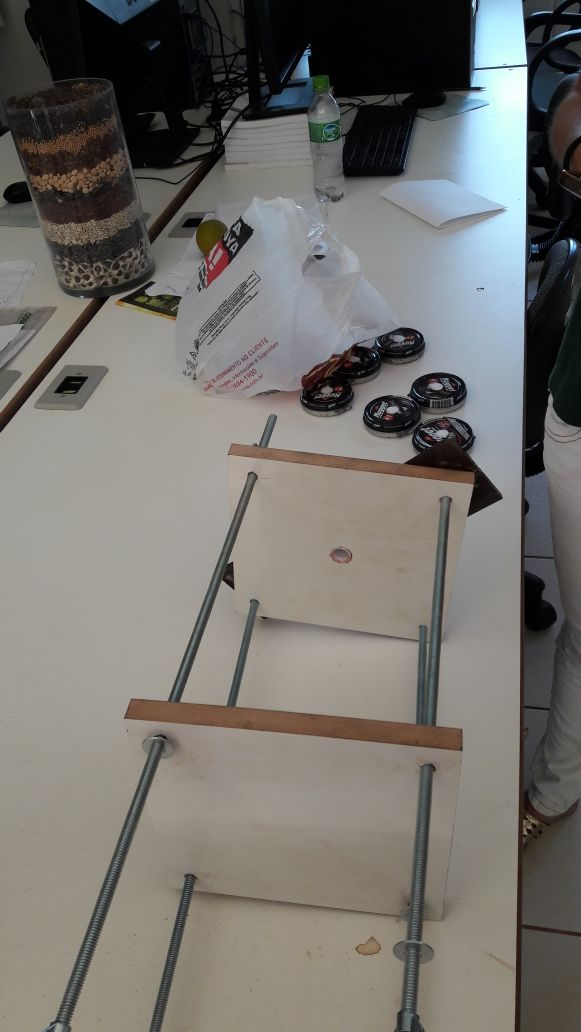
\includegraphics[width=\textwidth]{figuras/montagem1.png}
    \caption{Estrutura de madeira com os parafusos.}
  \end{subfigure}%
  \hfill
  \begin{subfigure}[H]{0.4\textwidth}
    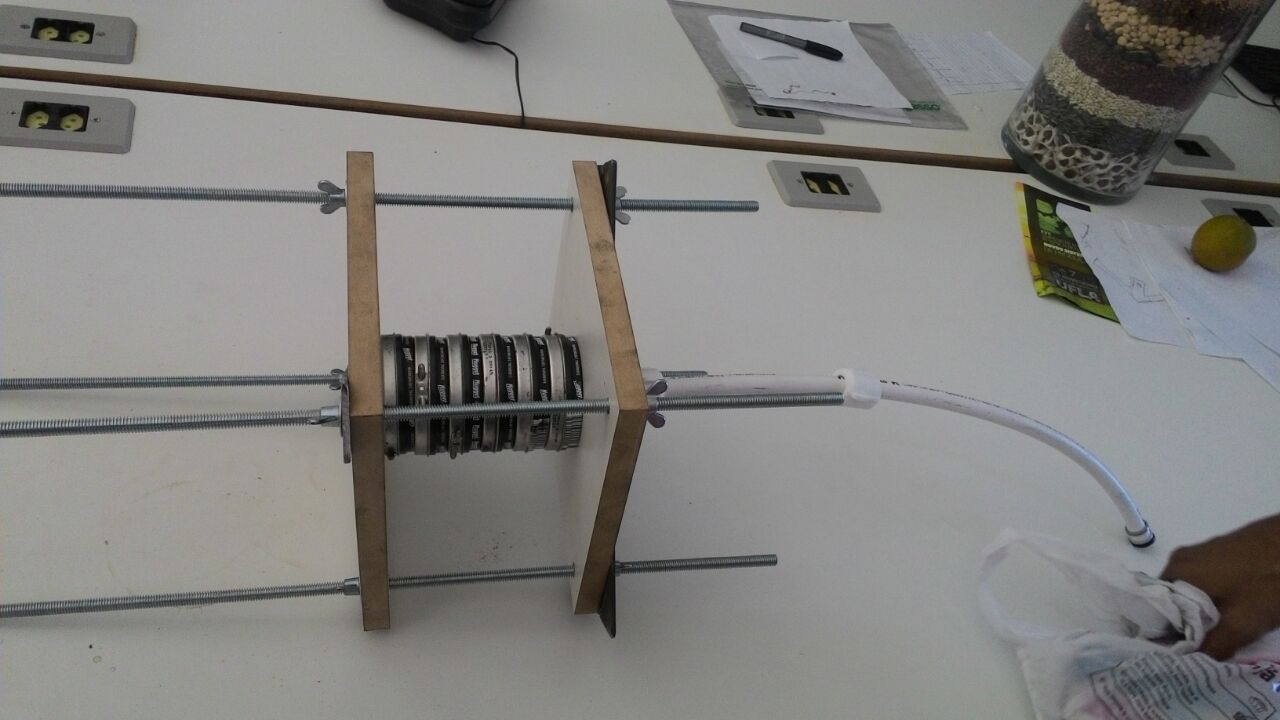
\includegraphics[width=\textwidth]{figuras/montagem2.png}
    \caption{Estrutura prensando as latas. A magueira branca é a alimentação.}
  \end{subfigure}%
  \caption{Montagem}
\end{figure}


%%% Local Variables:
%%% mode: latex
%%% TeX-master: "../main_archive"
%%% End:

\chapter{Resultados e Discussão}
\label{chap:resultados}


%%% Local Variables:
%%% mode: latex
%%% TeX-master: "../main_archive"
%%% End:

\chapter{Cronograma}
\label{chap:cronograma}

\begin{table}[H]
\label{cronograma}
\caption{Cronograma planejado}
\centering

\begin{tabular}{|P{6cm}|c|c|c|c|c|c|}
    \hline
    \multirow{2}*{\textbf{Atividades}} & \multicolumn{6}{c|}{\textbf{Semanas}} \\ \cline{2-7}
    & 1 & 2 & 3 & 4 & 5 & 6 \\
    \hline
    Revisão de literatura                & \textbf{X} & \textbf{X} & \textbf{X} &   &   &   \\
    \hline
    Preparação e separação dos materiais & \textbf{X} & \textbf{X} &   &   &   &   \\
    \hline
    Montagem do experimento              & \textbf{X} & \textbf{X} & \textbf{X} &   &   &   \\
    \hline
    Coleta de dados                      &   &   & \textbf{X} & \textbf{X} & \textbf{X} &   \\
    \hline
    Apresentação do projeto              &   &   &   &   &   & \textbf{X} \\
    \hline
    
\end{tabular}

\end{table}

%%% Local Variables:
%%% mode: latex
%%% TeX-master: "../main_archive"
%%% End:

%==============================================================================

% Incluindo bibliografia
%\bibliographystyle{plain}             % estilo para labels em numeros
%\bibliographystyle{alpha}             % estilo para labels em iniciais
\bibliographystyle{abntex2-num}         %% estilo para referências usando ABNT, 
 %para usar o abntex2-alf precisa arrumar o nome dos autores na bibliografia
%\bibliographystyle{abntex2-alf}           % estilo para referências usando ABNT, 

%inclui Referências Bibliográficas
\referencias
\bibliography{bibliografia/b}

%==============================================================================
% Fim do texto
\end{document}

%%% Local Variables:
%%% mode: latex
%%% TeX-master: t
%%% End:
